%*****************************************
\chapter{Visualizing Frequency}\label{vfr:visualizing_frequency}
%*****************************************
%TODO Reviewed

\section{Introduction}

Nominal and Ordinal data items are normally reported in frequency tables where the number of times a particular survey item was selected by respondents is displayed. However, there are many ways to visualize frequency data and many people find various charts and graphs to be useful. This lab introduces the visualization tools available in \texttt{SOFA}.

\section{Visualizing Data}

\subsection{Histogram} A histogram is a graph that shows how often various responses were selected on a survey. These are often presented as a graphic representation of the statistical data found in a frequency table in order to aid in understanding. Histograms are only used for data that are interval or ratio in nature, for example, age or height. Histograms are especially useful for interval or ratio data since \texttt{SOFA} will automatically cluster the data into ``bins.''

As an example of a histogram, Figure \ref{vfr:img01} shows the mother's age from the \textit{births} dataset.

\begin{figure}[H]
  \begin{center}
    \fbox{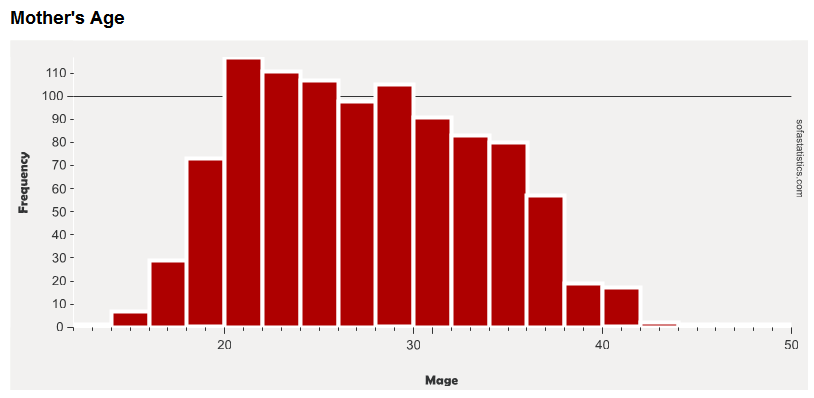
\includegraphics[width=0.95\linewidth]{gfx/vfr005}}
    \caption{Histogram of Mother's Age}
    \label{vfr:img01}
  \end{center}
\end{figure}

Notice that there is not a separate bar for each age; rather, \texttt{SOFA} has clustered two years into the same bar. Thus, there is a bar that combines $ 20 $-$ 21 $ and not separate bars for $ 20 $ and $ 21 $.

As another example, Figure \ref{vfr:img02} shows a histogram for baby's weight from the \textit{births} dataset.\footnote{Using a histogram aids a researcher in determining if a dataset is normally distributed and skewed. Figure \ref{vfr:img02} shows a normally distributed dataset since there is a clear peak in the middle trailing off on both sides. It also shows a negative skew since the tails on the left side of the peak are longer. Lab \ref{int:normal_distribution} on page \pageref{int:normal_distribution} discusses the shape of a normal distribution.}

\begin{figure}[H]
  \begin{center}
    \fbox{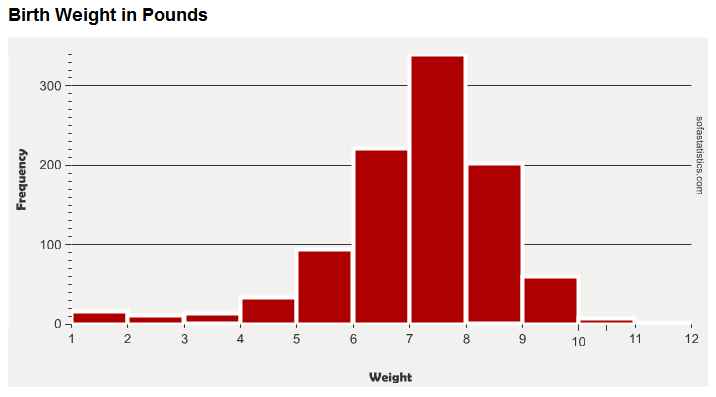
\includegraphics[width=0.95\linewidth]{gfx/vfr010}}
    \caption{Histogram of Baby's Weight}
    \label{vfr:img02}
  \end{center}
\end{figure}

As in Figure \ref{vfr:img01}, any weight between $ 6 $ and $ 6.99 $ pounds is clustered in a single bar between $ 6 $ and $ 7 $.

\subsection{Bar Chart} A bar chart is used to display the frequency count for ordinal or nominal data. There are technical differences between a bar chart and a histogram but for the purposes of this lab manual they can be considered identical. Figure \ref{vfr:img03} is a bar chart showing the prevalence of various drive trains in the \textit{cars} dataset.

\begin{figure}[H]
  \begin{center}
    \fbox{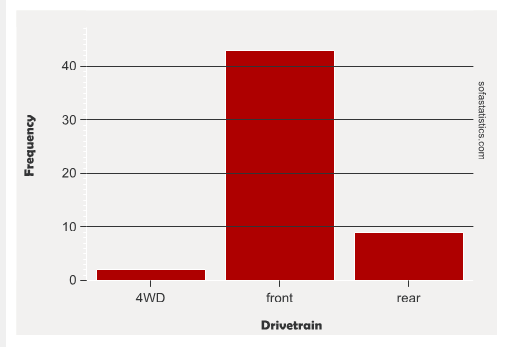
\includegraphics[width=.75\linewidth]{gfx/vfr015}}
    \caption{Prevelance of Types of Drive Trains}
    \label{vfr:img03}
  \end{center}
\end{figure}

Figure \ref{vfr:img04} shows the maturity level of the mothers in the \textit{births} dataset and unsurprisingly indicates that most mothers are younger.

\begin{figure}[H]
  \begin{center}
    \fbox{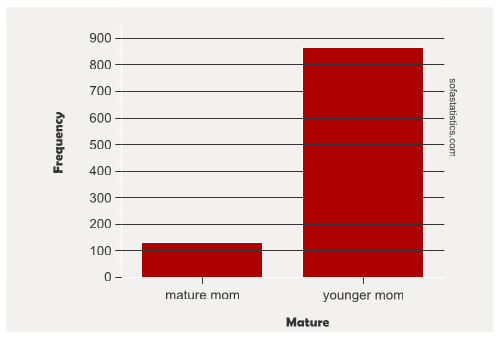
\includegraphics[width=.75\linewidth]{gfx/vfr020}}
    \caption{Maturity of Mothers}
    \label{vfr:img04}
  \end{center}
\end{figure}

\subsection{Clustered Bar Chart} A clustered bar chart displays two or more variables and is used to display ordinal or nominal data. In general, clustered bar charts can be difficult to interpret and should be avoided. Figure \ref{vfr:img05} is a clustered bar chart that shows the incidence of premature births by the mother's smoking habit in the \textit{births} dataset.

\begin{figure}[H]
  \begin{center}
    \fbox{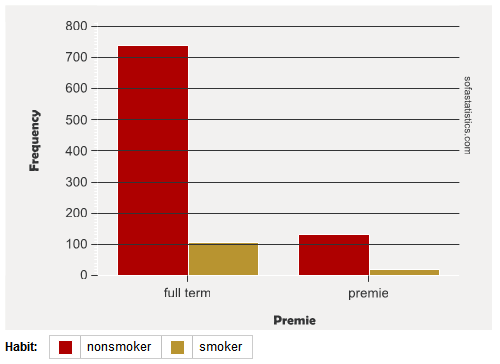
\includegraphics[width=0.95\linewidth]{gfx/vfr025}}
    \caption{Permature Births By Smoking Habit}
    \label{vfr:img05}
  \end{center}
\end{figure}

Figure \ref{vfr:img06} illustrates the problem with a clustered bar chart. This is a chart that shows the number of passengers for each type of car in the \textit{cars} dataset. Notice that no large cars have four or five passengers and no small cars have  six passengers so those bars are missing and that can make the chart difficult to interpret.

\begin{figure}[H]
  \begin{center}
    \fbox{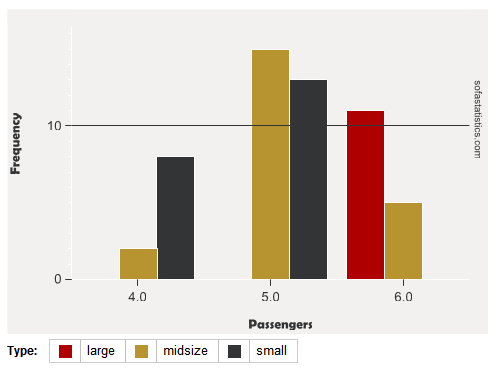
\includegraphics[width=0.95\linewidth]{gfx/vfr030}}
    \caption{Number of Passengers By Car Type}
    \label{vfr:img06}
  \end{center}
\end{figure}

\subsection{Pie Chart} A pie chart is commonly used to display nominal or ordinal data; however, pie charts are notoriously difficult to understand, especially if the writer uses some sort of $ 3 $-D effect or ``exploded'' slices. The human brain seems able to easily compare the \textit{heights} of two or more bars, as in histograms and bar charts, but the \textit{areas} of two or more slices of a pie chart are difficult to compare. For this reason, pie charts should be avoided in research reports. If they are used at all, they should only illustrate one slice's relationship to the whole, not comparing one slice to another; and no more than four or five slices should be presented on one chart.

Figure \ref{vfr:img07} shows the types of numbers found in messages in the \textit{email} dataset. This pie chart is easy to interpret since there are only three slices and each slice is easy to compare to the whole.

\begin{figure}[H]
  \begin{center}
    \fbox{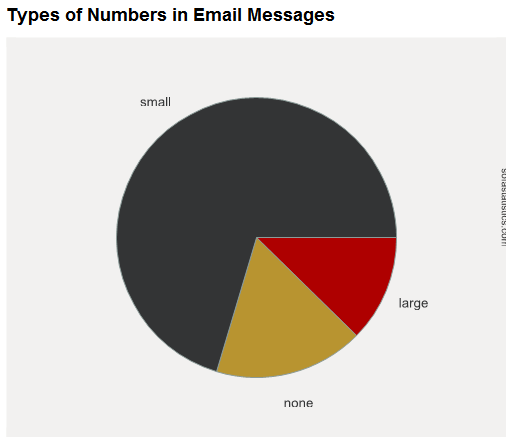
\includegraphics[width=0.7\linewidth]{gfx/vfr035}}
    \caption{Types of Numbers in Email Messages}
    \label{vfr:img07}
  \end{center}
\end{figure}

As an extreme example of a poorly used pie chart, consider Figure \ref{vfr:img08}. Even ignoring the problem of the numbers overlapping, making them impossible to read, the slices are so numerous and small that it is impossible to differentiate between them. For example, the ``one'' and ``two'' slices are impossible to compare. For this pie chart, about all that can be stated is that most email messages have zero dollar signs.

\begin{figure}[H]
  \begin{center}
    \fbox{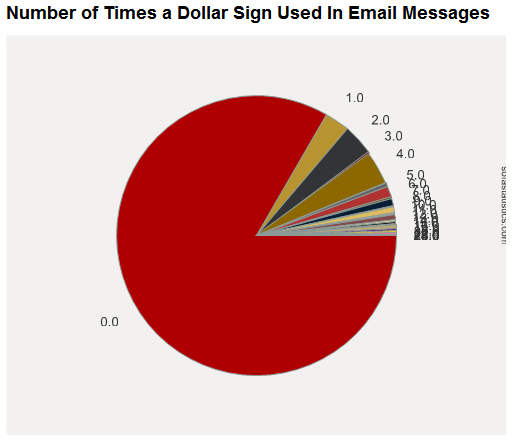
\includegraphics[width=0.7\linewidth]{gfx/vfr040}}
    \caption{Number of Times a Dollar Sign Used in Email Messages}
    \label{vfr:img08}
  \end{center}
\end{figure}

\subsection{Line Charts}

Line charts display the frequency of some value in a linear form that makes trend detection easier. As an example, consider the following from the \textit{gifted} dataset which charts the number of hours that parents spent reading to their children.

\begin{figure}[H]
  \begin{center}
    \fbox{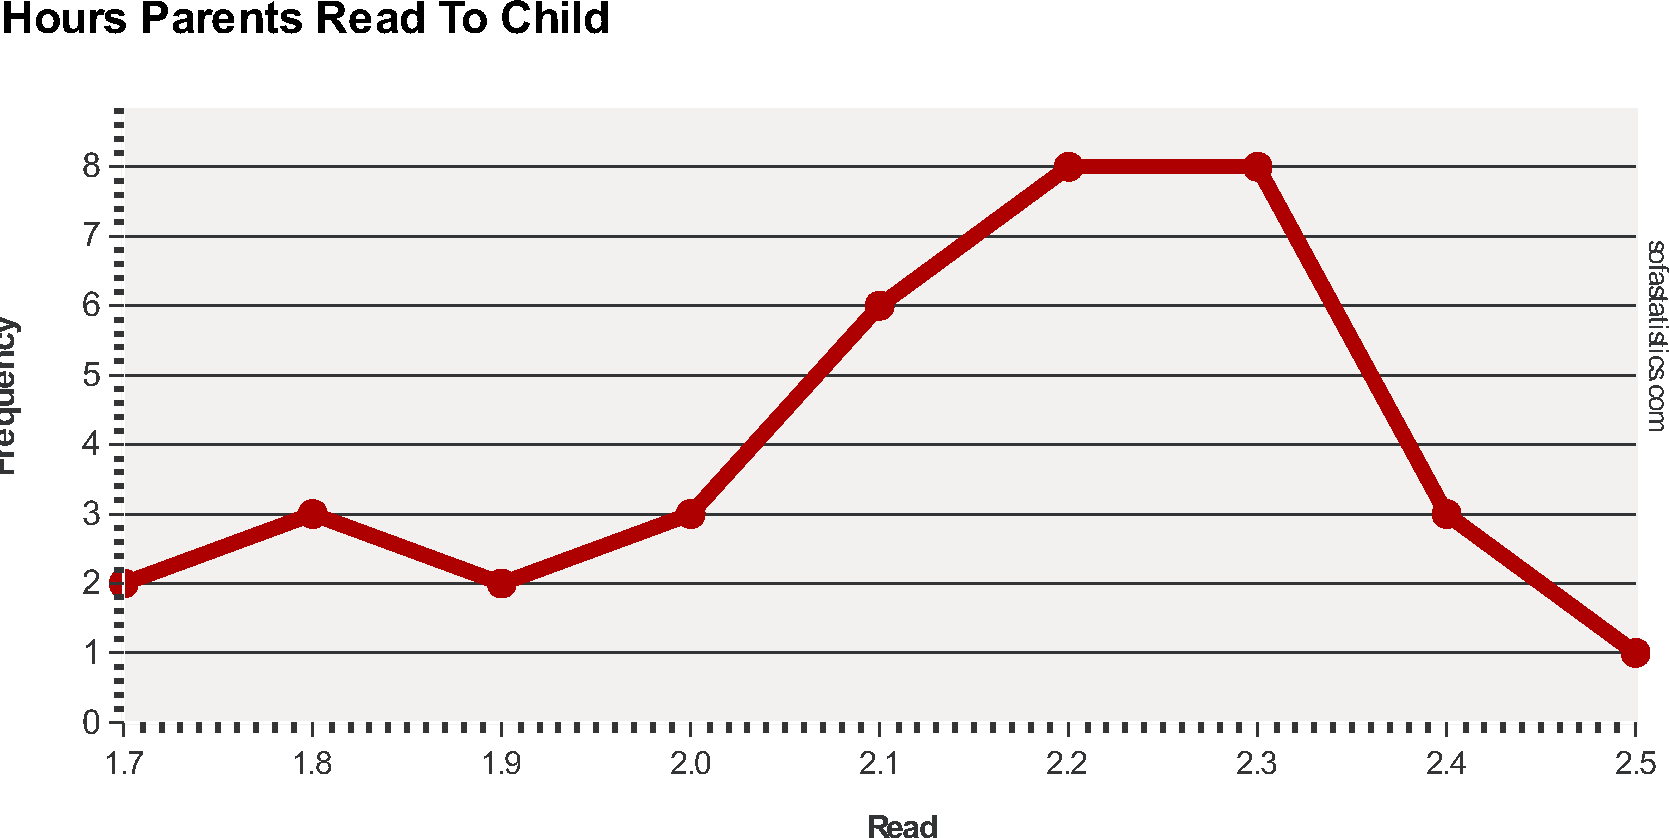
\includegraphics[width=0.95\linewidth]{gfx/vfr045}}
    \caption{Hours Spent Reading}
    \label{vfr:img08a}
  \end{center}
\end{figure}

This chart makes it easy to see that most parents in this survey read to their children about $ 2.2-2.3 $ hours per week. 

\section{Procedure}

Start \texttt{SOFA} and select ``Charts.'' Then:

\subsection{Histogram}

\begin{enumerate}
  \item Data Source Table: bdims
  \item Table Type: Histogram (sixth button)
  \item Values: Age 
  \item Title: Age Statistics
  
  \begin{figure}[H]
    \begin{center}
      \fbox{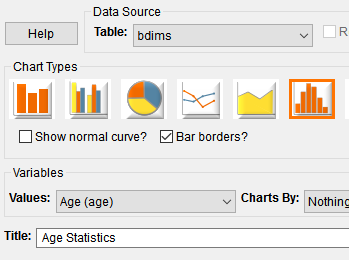
\includegraphics[]{gfx/vfr050}}
      \caption{Setting Up Age Statistics}
    \end{center}
  \end{figure}
  
  \begin{figure}[H]
    \begin{center}
      \fbox{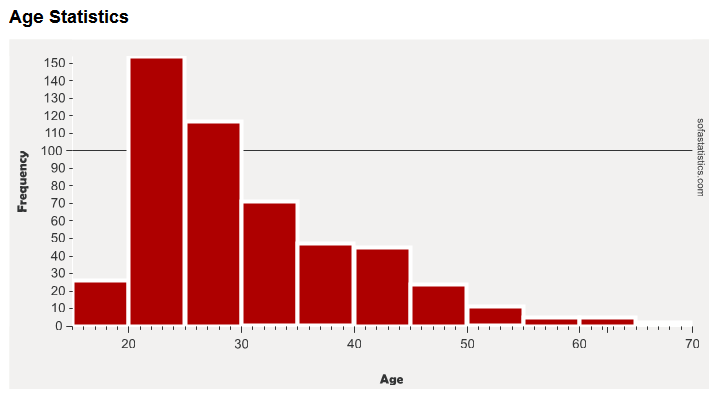
\includegraphics[width=0.95\linewidth]{gfx/vfr055}}
      \caption{Age Statistics}
    \end{center}
  \end{figure}
  
\end{enumerate}

\subsection{Activity 1: Histogram} \label{vfr:act01}

Using the \textit{maincafe} dataset in \texttt{SOFA}, produce an histogram of Age. The histogram should have a title of ``Visualizing Frequency, Activity 1'' and a subtitle of ``Histogram of Age''.

\subsection{Line Charts}

To create a line chart:

Start \texttt{SOFA} and select ``Charts'' then:

\begin{enumerate}
  
  \item Data Source Table: gifted
  \item Table Type: Line Chart (fourth button)
  \item Values: Read
  \item Title: Hours Parents Read To Child
  
  \begin{figure}[H]
    \begin{center}
      \fbox{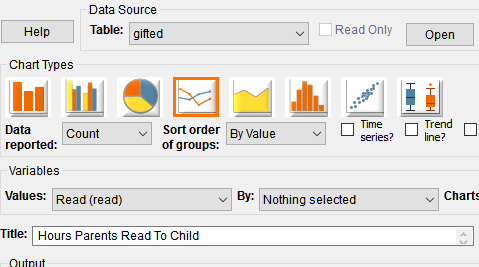
\includegraphics[width=0.95\linewidth]{gfx/vfr060}}
      \caption{Setting Up Line Chart}
    \end{center}
  \end{figure}

  \begin{figure}[H]
    \begin{center}
      \fbox{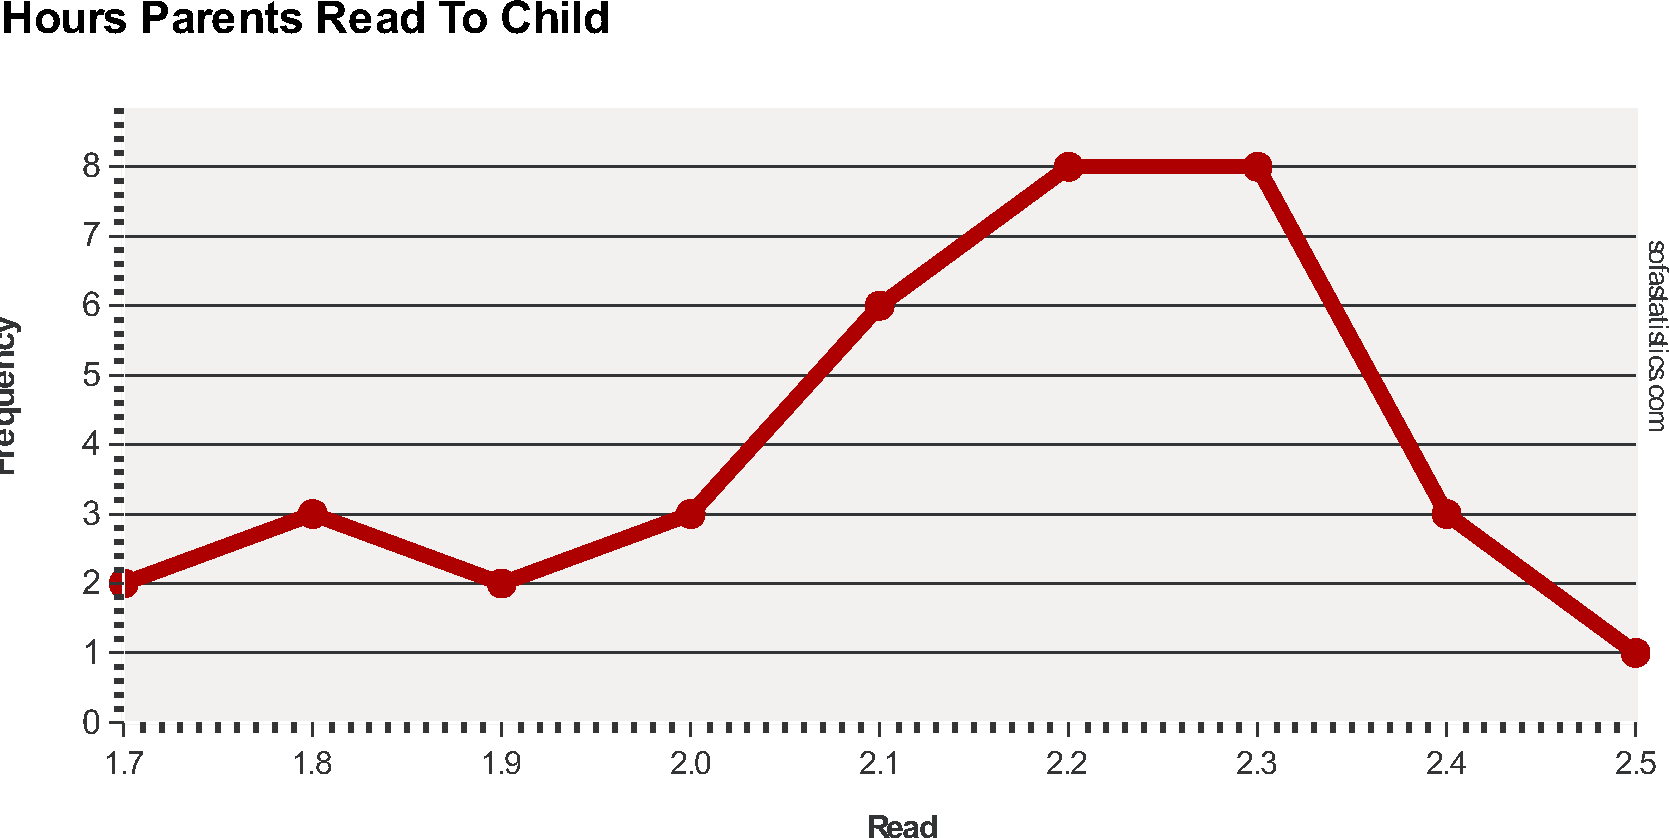
\includegraphics[width=0.95\linewidth]{gfx/vfr065}}
      \caption{Line Chart For Time Parents Spend Reading To Children}
    \end{center}
  \end{figure}
  
\end{enumerate}

If a ``By'' value is selected then a new line will be generated for each of the levels in the ``By'' variable. For example:

\begin{enumerate}
  \item Data Source Table: births
  \item Table Type: Line Chart (fourth button)
  \item Values: Mage
  \item By: Gender
  \item Title: Mother's Age and Baby Gender
  
  \begin{figure}[H]
    \begin{center}
      \fbox{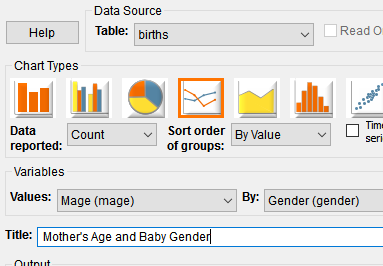
\includegraphics[]{gfx/vfr070}}
      \caption{Setting Up Line Chart}
    \end{center}
  \end{figure}
  
  \begin{figure}[H]
    \begin{center}
      \fbox{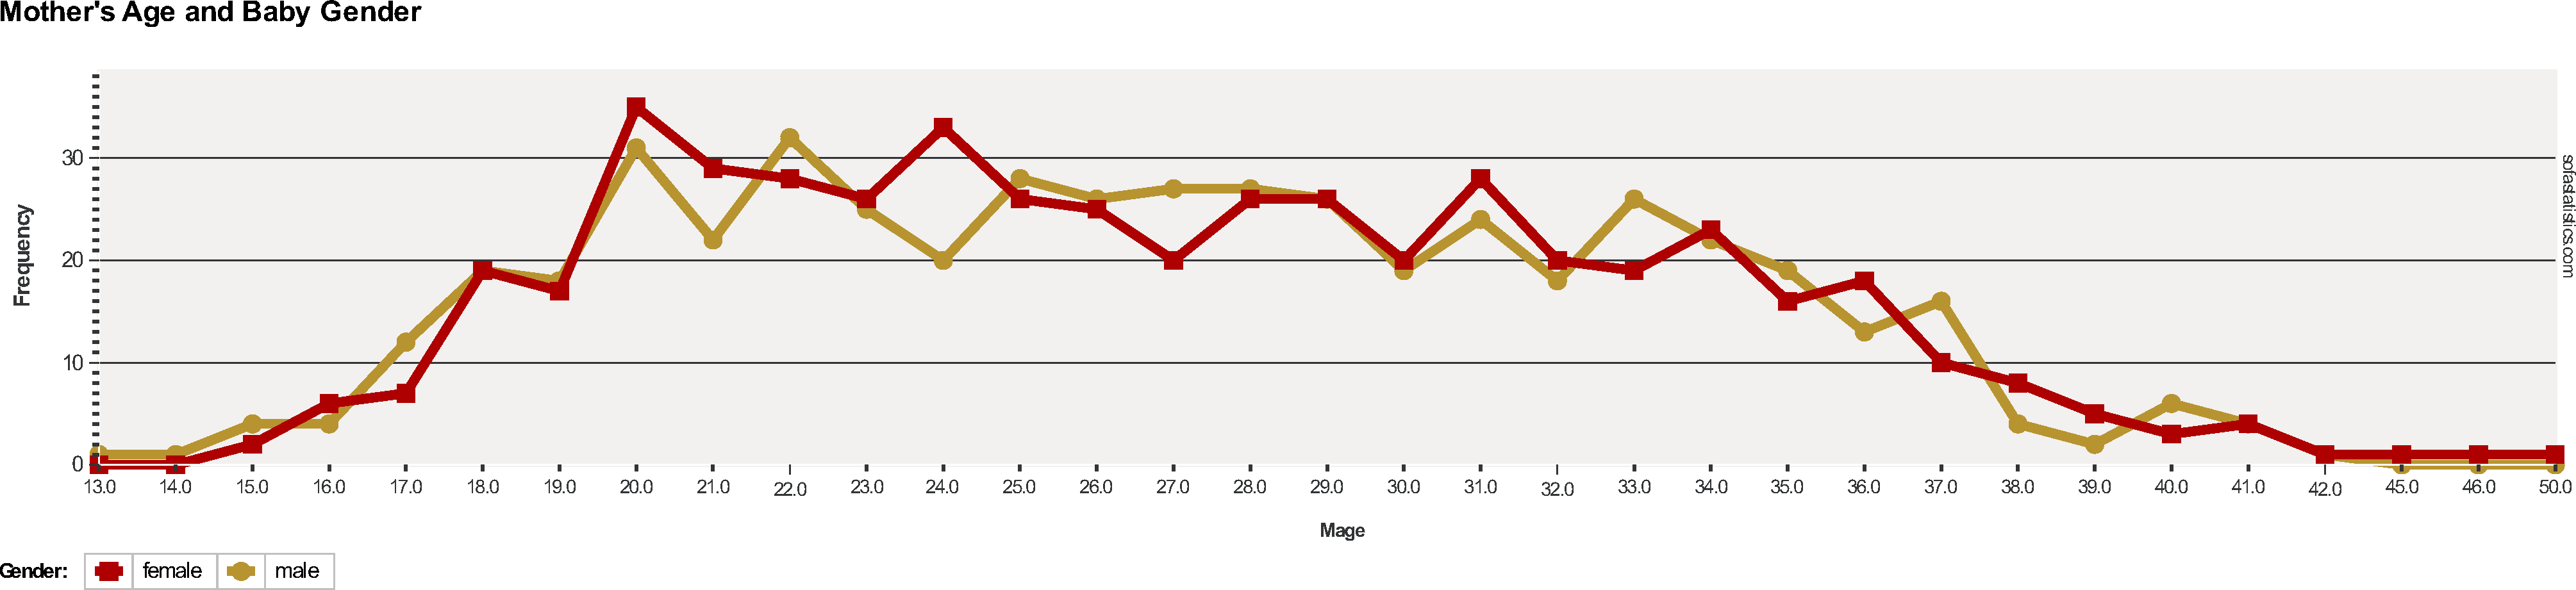
\includegraphics[width=0.95\linewidth]{gfx/vfr075}}
      \caption{Line Chart For Mother's Age and Baby Gender}
    \end{center}
  \end{figure}
\end{enumerate}

An ``Area Chart'' (button five) is the same as a line chart but the area under the line is colored which may make it easier to see trends. 

\begin{enumerate}
  \item Data Source Table: births
  \item Table Type: Area Chart (fifth button)
  \item Values: Mage
  \item Title: Mother's Age
  
  \begin{figure}[H]
    \begin{center}
      \fbox{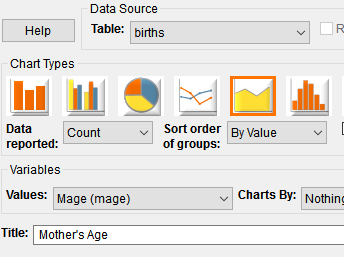
\includegraphics[]{gfx/vfr080}}
      \caption{Setting Up Area Chart}
    \end{center}
  \end{figure}
  
  \begin{figure}[H]
    \begin{center}
      \fbox{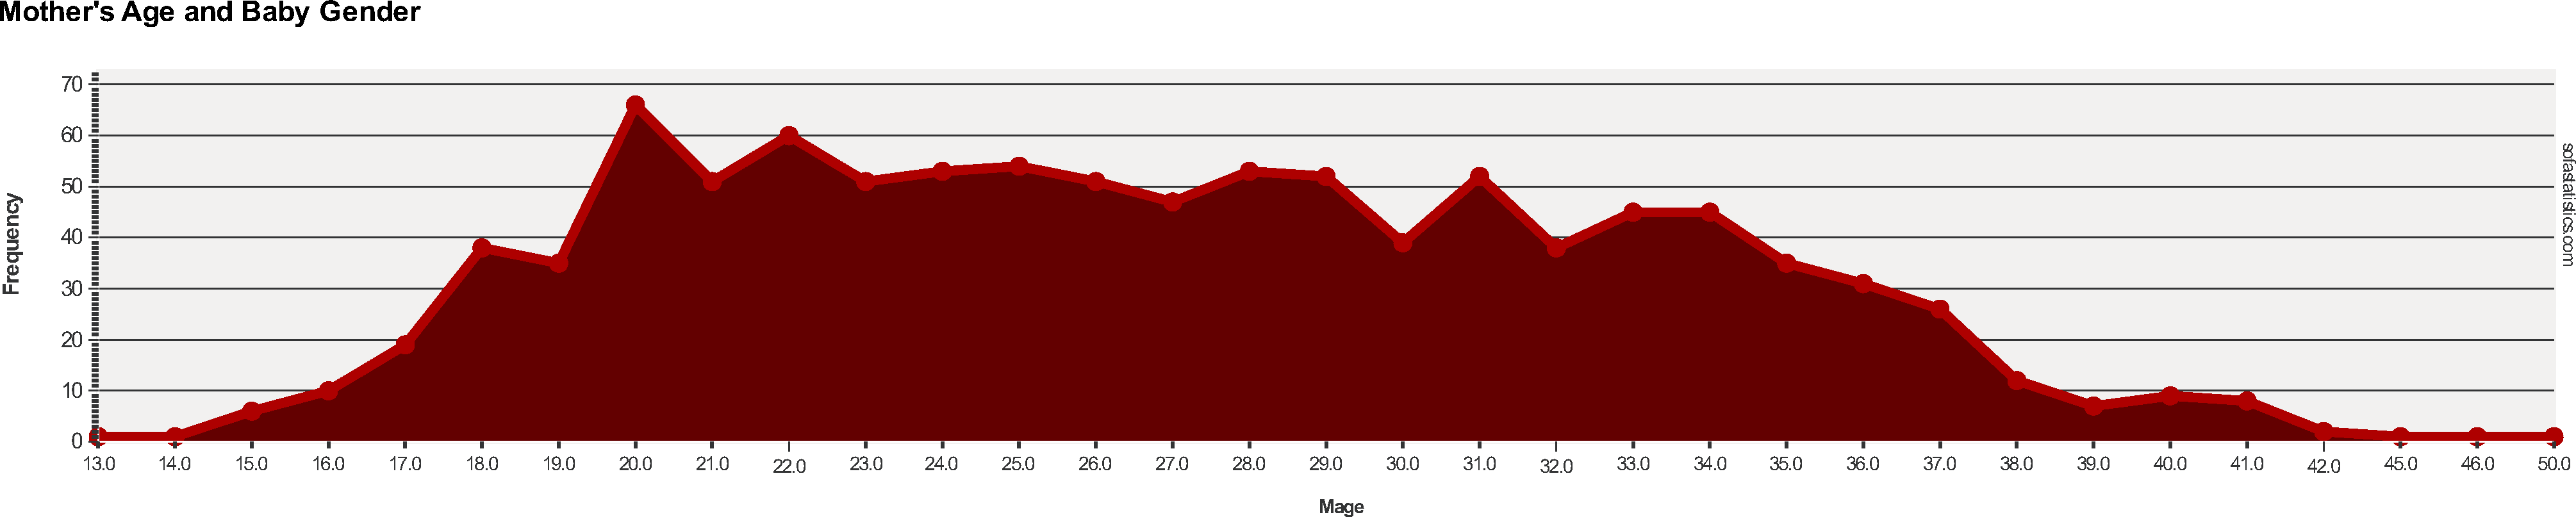
\includegraphics[width=0.95\linewidth]{gfx/vfr085}}
      \caption{Area Chart For Mother's Age}
    \end{center}
  \end{figure}
\end{enumerate}

Occasionally, data are in a ``time series'' where some observation was made over a period of time and \texttt{SOFA} is able to create line charts that display time series data.

\begin{enumerate}
  \item Data Source Table: doorsurvey
  \item Table Type: Line Chart (forth button)
  \item Options: Check the ``Time Series?'' button
  \item Dates/Times: Day
  \item Title: Customer Counts
  
  \begin{figure}[H]
    \begin{center}
      \fbox{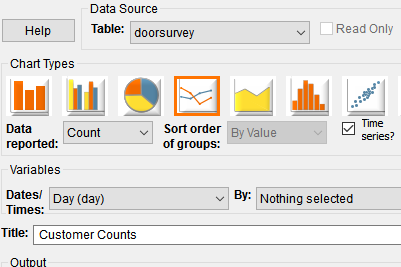
\includegraphics[]{gfx/vfr090}}
      \caption{Setting Up Time Series Chart}
    \end{center}
  \end{figure}
  
  \begin{figure}[H]
    \begin{center}
      \fbox{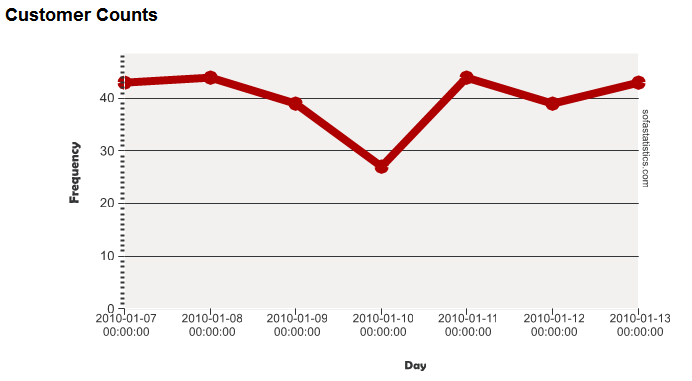
\includegraphics[width=0.95\linewidth]{gfx/vfr095}}
      \caption{Time Series Chart For Customer Counts}
    \end{center}
  \end{figure}
\end{enumerate}

\texttt{SOFA} is also able to display more than one time series on the same chart. For example, to display the number of customers by sex:

\begin{enumerate}
  \item Data Source Table: doorsurvey
  \item Table Type: Line Chart (forth button)
  \item Options: Check the ``Time Series?'' button
  \item Dates/Times: Day
  \item By: Gender
  \item Title: Customer Counts By Gender
  
  \begin{figure}[H]
    \begin{center}
      \fbox{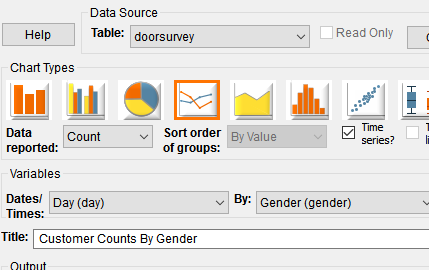
\includegraphics[]{gfx/vfr100}}
      \caption{Setting Up Time Series Chart By Sex}
    \end{center}
  \end{figure}
  
  \begin{figure}[H]
    \begin{center}
      \fbox{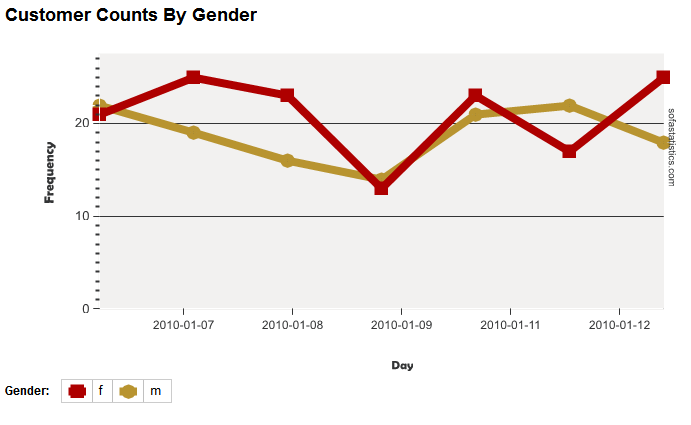
\includegraphics[width=0.95\linewidth]{gfx/vfr105}}
      \caption{Time Series Chart For Customer Counts By Gender}
    \end{center}
  \end{figure}
\end{enumerate}

\texttt{SOFA} includes a number of options for line charts that can be selected with the check boxes under the Chart Types buttons:

\begin{itemize}
  \item \textbf{Trend Line?} is a straight line added to a time series chart to help visualize a variable's trend over time.
  \item \textbf{Smooth Line?} produces a smoothed-out line rather than jagged.
  \item \textbf{Rotate Labels?} makes longer labels fit the chart space better.
  \item \textbf{Hide Markers?} removes the ``dots'' from the line.
  \item \textbf{Major Labels Only?} condenses the chart by only showing the major time divisions.
\end{itemize}

\subsection{Activity 2: Line Chart} \label{vfr:act02}

Using the \textit{maincafe} dataset in \texttt{SOFA}, produce a line chart of Ptysize by Sex. The line chart should have a title of ``Visualizing Frequency, Activity 2'' and a subtitle of ``Line Chart of Party Size by Sex''.

\subsection{Bar Chart}

\begin{enumerate}
  \item Data Source Table: cars
  \item Table Type: Bar Chart (first button)
  \item Values: Passengers 
  \item Title: Passengers
  
  \begin{figure}[H]
    \begin{center}
      \fbox{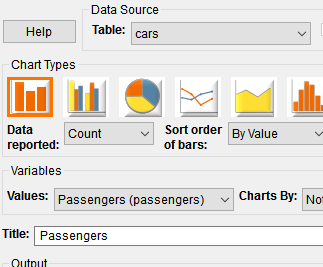
\includegraphics[]{gfx/vfr110}}
      \caption{Setting Up Passengers}
    \end{center}
  \end{figure}
  
  \begin{figure}[H]
    \begin{center}
      \fbox{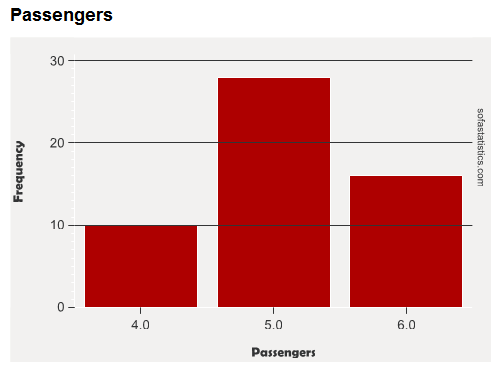
\includegraphics[width=0.95\linewidth]{gfx/vfr115}}
      \caption{Passengers}
    \end{center}
  \end{figure}
  
\end{enumerate}

\subsection{Activity 3: Bar Chart} \label{vfr:act03}

Using the \textit{maincafe} dataset in \texttt{SOFA}, produce a bar chart of Meal. The bar chart should have a title of ``Visualizing Frequency, Activity 3'' and a subtitle of ``Bar Chart of Meal''.

\subsection{Clustered Bar Chart}

\begin{enumerate}
  \item Data Source Table: cars
  \item Table Type: Clustered Bar Chart (second button)
  \item Values: Passengers 
  \item By: Drivetrain
  \item Title: Passengers By Drive Train
  
  \begin{figure}[H]
    \begin{center}
      \fbox{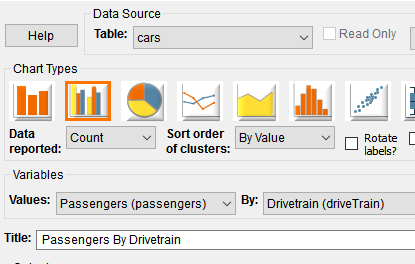
\includegraphics[]{gfx/vfr120}}
      \caption{Setting Up Passengers By Drivetrain}
    \end{center}
  \end{figure}
  
  \begin{figure}[H]
    \begin{center}
      \fbox{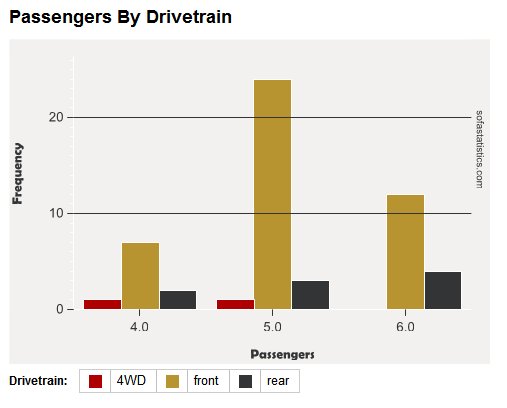
\includegraphics[width=0.95\linewidth]{gfx/vfr125}}
      \caption{Passengers By Drivetrain}
    \end{center}
  \end{figure}
  
\end{enumerate}

\subsection{Activity 4: Clustered Bar Chart} \label{vfr:act04}

Using the \textit{maincafe} dataset in \texttt{SOFA}, produce a clustered bar chart of Meal by Sex. The bar chart should have a title of ``Visualizing Frequency, Activity 4'' and a subtitle of ``Bar Chart of Meal by Sex''.

\subsection{Pie Chart}

\begin{enumerate}
  \item Data Source Table: cars
  \item Table Type: Pie Chart (third button)
  \item Values: Passengers 
  \item Title: Passengers
  
  \begin{figure}[H]
    \begin{center}
      \fbox{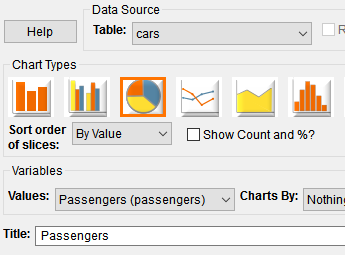
\includegraphics[]{gfx/vfr130}}
      \caption{Setting Up Passengers}
    \end{center}
  \end{figure}
  
  \begin{figure}[H]
    \begin{center}
      \fbox{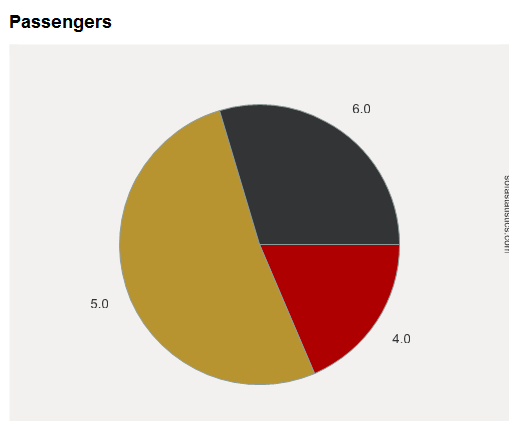
\includegraphics[width=0.8\linewidth]{gfx/vfr135}}
      \caption{Passengers}
    \end{center}
  \end{figure}
  
\end{enumerate}

\subsection{Activity 5: Pie Chart} \label{vfr:act05}

Using the \textit{maincafe} dataset in \texttt{SOFA}, produce a pie chart of Food. The pie chart should have a title of ``Visualizing Frequency, Activity 5'' and a subtitle of ``Pie Chart of Food''.

\section{Deliverable}

Complete the following activities in this lab:

\rowcolors{1}{gray!25}{}
\begin{center}
  \begin{tabular}{lll}
    \hline 
    \textbf{Number} & \textbf{Name} & \textbf{Page} \\ 
    \hline 
    \ref{vfr:act01} & \nameref{vfr:act01} & \pageref{vfr:act01} \\ 
    \ref{vfr:act02} & \nameref{vfr:act02} & \pageref{vfr:act02} \\ 
    \ref{vfr:act03} & \nameref{vfr:act03} & \pageref{vfr:act03} \\ 
    \ref{vfr:act04} & \nameref{vfr:act04} & \pageref{vfr:act04} \\ 
    \ref{vfr:act05} & \nameref{vfr:act05} & \pageref{vfr:act05} \\ 
    \hline 
  \end{tabular} 
\end{center}

Consolidate the responses for all activities into a single document and submit that document for grading.






